
%*******************************************************************************
%***********************************    Background   *****************************
%*******************************************************************************
%!TEX root = 0.main.tex

\setcounter{page}{1}



%********************************** %First Section  **************************************
\section {Introduction and general background} 

\subsection{Introduction}

Neural Networks (NNs) are popular algorithms for regression and classification tasks. Taking as example classification tasks of mapping the image $I$ into its correct label $C_I$, neural networks perform multiple combinations of linear and non-linear transformations of the image $I$ to assign it a label in $\mathcal C$.  The first \textit{layer} of a neural network transforms the input image $I$ in a vector $\mathbf f_1$ through a function $\phi_1$. $\mathbf f_1$ is used as input of the following layer that transforms it in a second vector $\mathbf f_2$ through a second function $\phi_2$, and so on, until the original image $I$ is mapped into a label $C_I$ by the last, $n$-th layer of the neural network:
$$C_I = \phi_n \circ \phi_{n-1}\circ ... \phi_2\circ\phi_1 (I)$$
 Given a large \textit{training set} of labeled images, a neural network is capable of learning the optimal transformations $\phi_i$ that let it map the input image to its correct label. Since the functions $\phi_i$ have many degrees of freedom - even millions - a neural network is able to learn very complex transformations. This characteristic makes NNs the optimal tool for complex tasks such as image classification, image segmentation, speech recognition and natural language processing.
 
Convolutional Neural Networks (CNNs) are a specific class of neural networks whose layer structure has been specifically designed for image recognition and segmentation. For this purpose, they don't have all the degrees of freedom of a normal, \textit{fully connected} neural network described above: each layer of a CNN has been constrained to only learn transformations of the input that are \textit{invariant} to translation of the input. This means that if used in an image classification task, a translation of the input image will not result in a change of class. The function $\phi_i$ of a CNN are \textit{convolutions} with some kernel that was learned during the training phase. Thanks to their design, training of CNNs is faster - thanks to the smaller number of parameters to be learned compared to a fully connected NN -, it is easier -since there's no need of artificially \textit{augmenting} the dataset with translated copies of the same image -, and leads to very accurate results.

Spherical convolutional neural networks (SCNNs) are NNs that have been specifically designed to deal with spherical data, whose layer design makes them \textit{equivariant to rotations of the input}.  Examples of tasks where data is naturally represented on a sphere are (i) climate science, where data is sampled on the surface of the Earth, (ii) cosmology, where observations are naturally projected on a sphere centered around the observer (see Figure \ref{fig:cosmicradiation}), and (iii) virtual reality, where the images are represented on a sphere centered around the player. Being able to come up with designs that are equivariant to rotations brings with it all the advantages that traditional CNNs have brought for traditional (euclidean) image classification tasks: training is faster, easier and results are very accurate. The transformations $\phi_i$ that each layer of a SCNN performs is a \textit{spherical convolution} of the input vector with a kernel learned during the training phase. One of the main issues with traditional SCNNs is the computational complexity of computing at each layer the Spherical Harmonic Transform (SHT) of the data to perform the convolution in the spectral domain. Perraudin et al. \cite{DeepSphere} proposed a Graph Convolutional Neural Network (GCNN) that is almost equivariant to rotations, replacing the SHT with a more efficient Graph Convolution.
\begin{figure}
	\centering
	\caption{\label{fig:cosmicradiation} Cosmic microwave background map, the oldest electromagnetic radiation in the universe. Source: Wikipedia}
	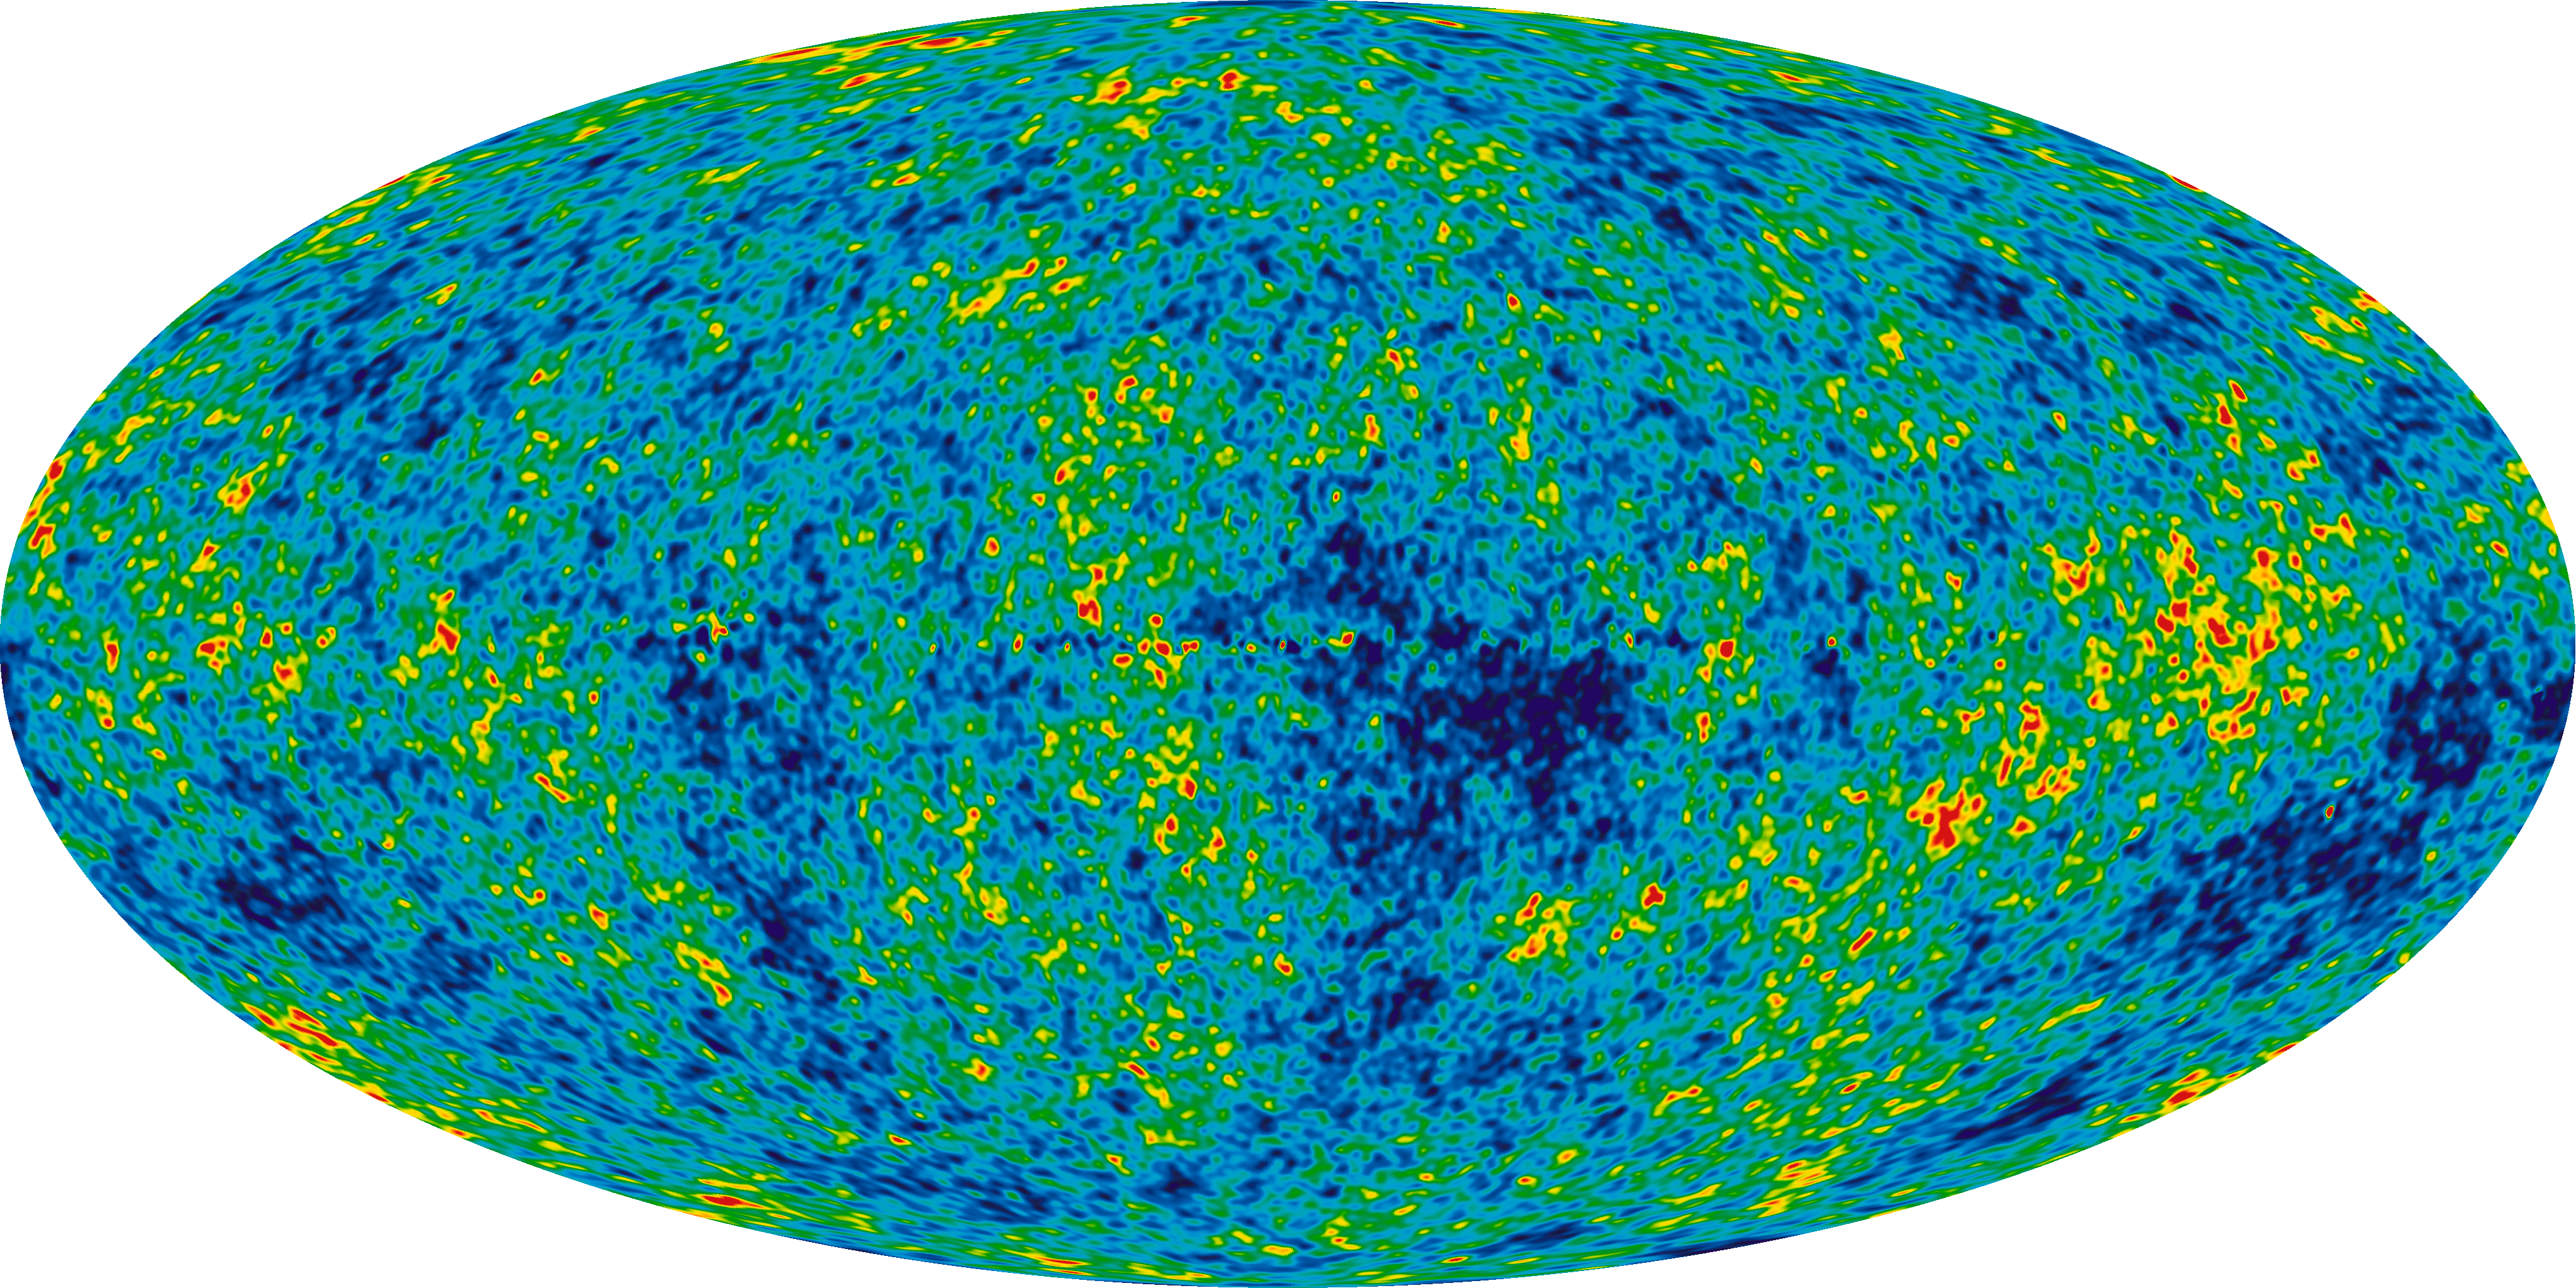
\includegraphics[width=0.4\textwidth]{figs/literaturereview/WMAP.png}
\end{figure}

In Chapter 1 we start by presenting fundamental concepts of spectral theory on the sphere and we present classical ways of building rotation equivariant neural networks through the use of the classical SHT.  We present then some basics of Graph Spectral Theory useful to introduce the work of Perraudin et al. DeepSphere \cite{DeepSphere}. We present then a well suited way to build a graph to approximate the Laplace-Beltrami operator on a manifold, the Heat Kernel Graph Laplacian (HKGL) together with some convergence results. In Chapter 2 we study the spectral properties of the graph Laplacian matrix $\mathbf L$ used by Perraudin et al. and we show a way to build a graph $G'$ such that the corresponding graph Laplacian matrix $\mathbf L'$ shows better spectral properties. In Chapter 3 we investigate other different methods of building the matrix $\mathbf L$ better suited to non uniform sampling measures. In particular, we study the Finite Element Method approximation of the Laplace-Beltrami operator on the sphere. We compare the FEM and the graph Laplacian on different samplings of the sphere. We conclude by discussing the general problem of how to incorporate geometrical informations about the sphere in the graph, a purely topological object.

\subsection{Fourier Transforms and Convolutions on the 2-Sphere}\label{sec:Fourier on the Sphere}
The goal of this section if to present to the reader some fundamental results of spectral theory on the sphere that we will need in this work. We start with a brief review Banach and Hilbert spaces, and we continue by defining the spherical harmonics, the fourier transform and the convolution on the sphere. We refer to Sections 2 and 3 of the work of Driscoll and Healy \cite{Driscoll:1994:CFT:184069.184073} for a more detailed and effective review of spectral theory on the Sphere.

\paragraph{Banach and Hilbert spaces}
A \textit{norm} $\norm\cdot:\ X\to\mathbb R$ on a vector space $X$ is a subadditive, positive definite function such that $\norm{x+y}\leq\norm x +\norm y,\ \forall x,y\in X$ (triangle inequality). A \textit{Cauchy sequence} $(x_n)\subset X$ is a sequence such that $\forall \epsilon>0\  \exists M>0: $ $\forall i,j>M$ $ \norm{x_i-x_j}<\epsilon$. A \textit{Banach space} $(X, \norm{\cdot})$ is a normed vector space on the scalar field $F$ that is \textit{complete}, meaning that $X$ is "big enough" such that for every Cauchy sequence $(x_n)\subset X$ there exist a $x\in X$ such that $x$ is the limit of $(x_n)$ in $X$ i.e. $\norm{x_n-x}\rightarrow 0$. A \textit{basis} of $(X, \norm\cdot)$ is a minimal set of linearly independent vectors $\mathcal B \subset X$ such that every element of $X$ can be written as linear combination of the elements of $\mathcal B$. For reasons that will be clear when presenting the Galerkin method, we are interested in those particular Banach spaces where we can define a notion of orthogonality between vectors. Such Banach spaces are called \textit{Hilbert spaces}: $(X, \norm \cdot )$ is a Hilbert space when it is Banach and furthermore the norm $ \norm \cdot $ can be induced by a \textit{scalar product}: $\norm \cdot = \sqrt{\langle\cdot,\cdot\rangle}$. A scalar product is a function $\langle\cdot,\cdot\rangle: X\times X \rightarrow \mathbb F$ that is linear in the first argument, positive definite and conjugate symmetric. Through a scalar product we can define the notion of angle $\theta$ between two elements $x, y \in X$ through the following formula: 
$$
\cos \theta = \frac{\langle x, y\rangle}{\norm x \norm y}
$$ 
and in particular we can define the notion of orthogonality: two elements  $x, y \in X$ are orthogonal if and only if $\langle c, y\rangle=0$. We can now define what an \textit{orthonormal} basis of $X$ is: a basis $\mathcal B \subset X$ such that $\forall x, y \in \mathcal B, \norm x = \norm y = 1 \text{and } \langle x, y\rangle = 0$. Given an orthonormal basis $\mathcal B = \{b_i\}_{i\in I}$ we can write each vector in its \textit{Fourier series} 
\begin{equation}\label{eq:abstract fourier}
x = \sum_{i\in I} \frac{\langle x, b_i\rangle}{\norm {x^2}}b_i
\end{equation}
If the set $I$ is countable the Hilbert space $(X, \norm\cdot)$ is called \textit{separable}. Having a countable orthonormal basis, and thus the possibility of representing each vector through its Fourier series enormously simplifies many problems.
\paragraph{Spherical Harmonics}
 Given the usual parametrization $x = x(\theta, \phi), \theta\in[0,\pi], \phi\in[0,2\pi]$ of the sphere
\begin{align*}
\mathbb{S}^{2}&=\left\{\omega=\left(\omega_{1}, \omega_{2}, \omega_{3}\right) \in \mathbb{R}^{3} :\|x\|_{\mathbb{R}^{3}}=\left(\omega_{1}^{2}+\omega_{2}^{2}+\omega_{3}^{2}\right)^{1 / 2}=1\right\}\\
\omega_{1}&=\cos (\phi) \sin (\theta), \quad \omega_{2}=\sin (\phi) \sin (\theta), \quad \omega_{3}=\cos (\theta)
\end{align*}
the Hilbert space $L^2(\mathbb S^2)$ is defined as the space of square-integrable functions endowed with the scalar product $\langle f,g\rangle=\int_{\mathbb S^2}f(\omega)\overline g(\omega)d\omega$ where the measure $d\omega$ is the rotation-invariant measure such that
\begin{align}
\int_{\omega \in \mathbb S^{2}} f(\omega) d \omega&=\int_{\phi=0}^{2 \pi} \int_{\theta=0}^{\pi} f(\omega(\theta, \phi)) \sin \theta d \theta d \phi\\
\int_{\omega \in \mathbb S^{2}} f(g \omega) d \omega&=\int_{\omega \in \mathbb S^{2}} f(\omega) d \omega, \quad g \in S O(3)
\end{align}

For each rotation $g\in SO(3)$ we define a corresponding rotation operator $\Lambda(g)$ by
$$
\Lambda(g) f(\omega)=f\left(g^{-1} \omega\right)
$$
A space is invariant under the rotations $g$ in $SO(3)$ if all operators $\Lambda(g)$ take each function of the space back into the space. As very well written by Driscoll et al \cite{Driscoll:1994:CFT:184069.184073}:

\vspace{0.2cm}
\textit{Fourier analysis on the sphere amounts to the decomposition of the space of square integrable functions on \(\mathbb S^{2}\) in minimal subspaces invariant under all of the rotations in \(S O(3),\) thus simplifying the analysis of rotation-invariant operators.}
\vspace{0.2cm}

The $\ell$-th invariant subspace is made of polynomials of $\mathbb R^3$ restricted to the sphere of degree $\ell$ and has dimension $2\ell+1$. The invariant space of degree $\ell$ is called the space of \textit{spherical harmonics} of degree $\ell$. These subspaces are orthogonal between them, and correspond to the eigenspaces of the Laplace-Beltrami operator $\Delta_{\mathbb S^2}$. The set of all the orthonormal basis $Y_\ell^m,\ -\ell\leq m\leq\ell$ of each minimal invariant subspace gives an orthonormal basis of $L^2(\mathbb S^2)$. The analytical expression of the spherical harmonic $Y_\ell^m(\theta, \phi)$ is known:
\begin{equation}\label{eq:spherical harmonics}
	Y_\ell^m(\theta, \phi) = (-1)^{m} \sqrt{\frac{(2 \ell+1)(\ell-m) !}{4 \pi(\ell+m) !}} P_{\ell}^{m}(\cos \theta) e^{i m \phi}
\end{equation}
where the definition of the Legendre functions $P_{\ell}^{m}$ can be found in \cite{Driscoll:1994:CFT:184069.184073}. 
\vspace{0.5cm}
\begin{remark}
	Saying that the space $V_\ell$ of spherical harmonics of degree $\ell$ is invariant under rotations $SO(3)$ means that under any rotation $g\in SO(3)$, any spherical harmonic $Y_\ell^m\in V_\ell$ is transformed into a linear combination of the others spherical harmonics of the same degree $\ell$:
	$$
	\Lambda(g) Y_{\ell}^{m}(\omega)=\sum_{|k| \leq \ell} Y_{\ell}^{k}(\omega) D_{k, m}^{(\ell)}(g)
	$$
\end{remark}
\vspace{0.5cm}

\paragraph{Fourier transform}
We can now expand each function $f\in L^2(\mathbb S^2)$ in the coordinate system given by the spherical harmonics 
\begin{align}
	f(\omega) &= \sum_{\ell\in\mathbb N}\sum_{|m|\leq \ell}\hat f_\ell^mY_\ell^m(\omega)\\
	\hat f_\ell^m &=\int_{\omega\in\mathbb S^2}f(\omega)Y_\ell^m(\omega)d\omega
\end{align}
where the coefficients $\hat f_\ell^m$ are the \textit{Fourier coefficients} of $f$.

The fact that $Y_\ell^m(\theta, \phi)$ depends on $\phi$ through a purely imaginary exponential - equation \ref{eq:spherical harmonics} - makes it possible to decompose the computation of the SHT in the two directions, latitude and longitude, and to use standard one-dimensional FFT algorithms to compute the longitudinal part of the transform on samplings of the sphere where the pixels lie on isolatitude circles.

\paragraph{Convolutions}
Convolution on the sphere is profoundly different than convolution on the Euclidean plane. On $\mathbb R^2$ the convolution of two functions $f, g \in \L^2(\mathbb R^2)$ is itself a function of the same space:
$$ \int_{\mathbb R^2} f(x)g(x-y)dy = f\star g(x) \in L^2(\mathbb R^2)$$

On the sphere things work differently; translations are replaced by rotations. Translations are isomorphic to $\mathbb R^2$, but rotations are not isomorphic to the sphere and constitute the three dimensional manifold $SO(3)$. For this reason, if we define $f\star k$ as follows:
\begin{equation} \label{eq:cohen convolution}
f\star k(g) := \int_{\eta \in \mathbb S^2} \Lambda(g)k( \eta) f(\eta) d\eta=\int_{\eta \in \mathbb S^2} k(g^{-1} \eta) f(\eta) d\eta\\ 
\end{equation}
the result $f\star k(g)$ is not a function of the sphere anymore, but it is a function of the special rotation group $SO(3)$. Cohen et al. \cite{SCNN} use in their work this definition of convolution on the sphere to construct a rotation equivariant NN. However, the definition of convolution that we will use in this work and that is more similar to the convolution of graphs that we will introduce later is the following, where the integral is performed not on the sphere but on the rotation group $SO(3)$:

\begin{equation}\label{eq:convolution}
	\begin{aligned} H_{k} f(\omega) &=\left(\int_{g \in S O(3)} d g k(g \eta) \Lambda(g)\right) f(\omega) \\ &=\int_{R \in S O(3)} k(g \eta) f\left(g^{-1} \omega\right) d g \\ &=k * f(\omega) \end{aligned}
\end{equation}

where $dg$ can be written in terms of the three Euler angles $(\theta, \phi, \psi)$ 
$$dg=\sin\theta d\theta d\phi d\psi$$
In this way the result $k * f(\omega)$ is still a function defined on the sphere. However, integrating on $SO(3)$ means integrating on the third Euler angle $\psi$, that means that we can only use \textit{radial} kernels $k$ .
For definition (\ref{eq:convolution}) we have the following theorem:
\vspace{0.5cm}
\begin{theorem}
	Given two functions $f, g$ in $L^2(\mathbb S^2)$, the Fourier transform of the convolution is a pointwise product of the transforms
$$
\hat{(f * h)}(\ell, m)=2 \pi \sqrt{\frac{4 \pi}{2 \ell+1}} \hat{f}(\ell, m) \hat{h}(\ell, 0)
$$
\end{theorem}
\vspace{0.5cm}

\subsection{Spherical Convolutional Neural Networks}
Cohen et al. \cite{SCNN} proposed in their work a NN where the first layer performs a convolution on the sphere defined by equation \ref{eq:cohen convolution}. The output feature map - a signal on $SO(3)$ - is processed by the deeper layers that are designed to perform other convolutions but in $SO(3)$. Convolutions are performed in the spectral domain, meaning that every signal has to be Fourier-transformed. This approach, even with the use of Generalized FFT algorithms for the sphere and for $SO(3)$, remains computationally expensive. In table \ref{tab:SHREC17_class} Gusset et al. \cite{Gusset} compared both the training and inference time of Cohen's SCNN, showing how slow this architecture is compared to other rotation equivariant architectures.
\subsection{Graph Spectral Theory} \label{sec:Chapter1: Spectral Graph Theory}
\paragraph{Graphs}
For the purposes of this work, an undirected graph $G(V, E, \mathbf W)$ is defined by a vertex set $V$ and an edge set $E$, where the edges are unordered pairs of vertices weighted by the matrix $\mathbf W$ whose entries $w_{ij}$ represent the weight of the edge $(v_i, v_j)$: zero if there's no edge, positive otherwise. Undirected graphs are common mathematical objects used to model simple, symmetric relationships between things. An edge $e = (v_i, v_j) \in E$ is the mathematical translation of the fact that the object indexed by $i, j$ are in a some kind of relationship. Common examples are friendship graphs, where people are the vertices and the edges represent friendship, or electric network graphs, where vertices represent electronic components and edges represent wires.
\paragraph{The graph Laplacian}
Given a weight matrix $\mathbf W$, one can define the graph Laplacian to be the matrix $\mathbf L = \mathbf D-\mathbf W$ where $\mathbf D$ is the diagonal matrix $\mathbf D_ii = \sum_j w_{ij}$:
\begin{equation}\label{eq:graph Laplacian}
	(\mathbf{L})_{ij}=\begin{cases}
	\sum_k w_{ik} & \text{if }i=j\\
	-w_{ij}&\text{if }i\neq j
	\end{cases}
\end{equation}
and the normalized graph Laplacian
\begin{equation}\label{eq:normalized graph Laplacian}
\mathbf L' = \mathbf I - \mathbf D^{-1/2}\mathbf L\mathbf D^{-1/2}
\end{equation}
A quantity that is a function of the vertex set $V$, for example the age of people in a friendship graph, one can define a vector $\mathbf f$ such that each entry $\mathbf f_i$ is the age of the person associated with the i-th vertex. One could try to measure how much in a friendship network people tend to be friends with people of the same age; in other words, how smooth the signal $\mathbf f$ is on the graph. A measure for the smoothness of a signal on a graph is given by the quadratic form associated with the normalized Laplace operator $\mathbf L'$:
$$
\mathbf f^T \mathbf L' \mathbf f = \sum_{\left(v_{j}, v_{k}\right) \in {E}} \frac{\boldsymbol{W}_{j k}}{\sqrt{d_{j} {d}_{k}}}\left(\boldsymbol{f}_{j}-\boldsymbol{f}_{k}\right)^{2}
$$
\paragraph{Graph Fourier transform}
Since the normalized graph Laplacian is a symmetric matrix, its eigenvectors $V$ constitute an orthonormal basis of $\mathbb R^n$ and its eigenvalues are all real 
$$\mathbf L' = \mathbf V\mathbf \Lambda\mathbf V^T
$$
Similarly to the continuous domain, where the Fourier transform of a signal $f$ is defined as the projection of $f$ on the orthonormal eigenbasis of the Laplace-Beltrami operator $\Delta$, on a graph we can define a graph Fourier transform of a discrete signal $\mathbf f$ as the projection of $\mathbf f$ onto the eigenvectors of the normalized graph Laplacian $\mathbf L'$:
\begin{equation}\label{eq:graph fourier}
\mathcal F_G(\mathbf f) = \mathbf V^T\mathbf f = \hat{\mathbf f}
\end{equation}
The inverse graph Fourier transform is thus 
\begin{equation}\label{eq:graph fourier inverse}
\mathcal F^{-1}_G(\hat{\mathbf f}) = \mathbf V \hat{\mathbf f} = \mathbf V\mathbf V^T\mathbf f = {\mathbf f}
\end{equation}
\subsection{Deep Sphere V1.0}\label{sec:Chapter1:DeepSphere}
[TODO: Review of \textit{Deep Sphere}]
\subsubsection{HEALPix}\label{sec:Chapter1:HEALPix}
HEALPix is an acronym for Hierarchical Equal Area isoLatitude Pixelization of a sphere. This sampling produces a subdivision of the sphere in which each node covers the same surface area as every other node. It is parametrized by a parameter $N_{side}\in\mathbb N$, and is made by $n=12N_{side}^2$ nodes. The points of this sampling lie on isolatitude rings, that makes possible the implementation of an FFT algorithm for the discrete Fourier transform (also called in the case of the sphere Spherical Harmonic transform, SHT) of a sampled signal. The minimal resolution for HEALPix is given by $N_{side}=1$ and is made by 12 pixels. For each increasing value of $N_{side}$ each patch is divided into 4 equal area patches centered around the pixels of the new sampling (figure \ref{fig:healpix sampling})
\begin{figure}
	\centering
	\includegraphics[width=0.5\textwidth]{figs/chapter1/healpix.jpg}
	\caption{\label{fig:healpix sampling}HEALPix sampling for $N_{side}=1,2,3,4$}
\end{figure}
\subsection{Belkin's work}
[TODO: Review of Belkin's work]
